\subsection{MPU-6050 Accelerometer/Gyroskop}

MPU-6050 er en kombination af et accelerometer, et gyroskop, begge med 3 akser og et termometer. Det betyder for systemet at det er i stand til at registrere en ændring i acceleration og/eller orientering i alle retninger. Sensoren er blevet valgt til projektet på baggrund af et \IIC interface, som derved kan tilkobles en samlet bus sammen med andre sensorer på bilen. Udover dette giver det konstruerede breakoutboard mulighed for nem tilslutning, men fortsat lille størrelse på sensoren.
Sensoren fungerer altid som en slave med adressen $0b110100X$, hvor X bliver bestemt af det logiske niveau på pin AD0, der som standard er lav. 

\begin{figure}[h]
	\centering
	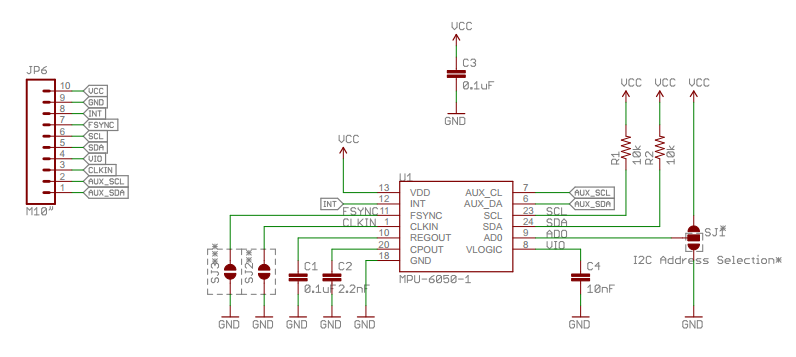
\includegraphics[width=\textwidth*4/5]{../fig/billeder/mpu6050.png}
	\caption{MPU-6050 diagram}
	\label{fig:mpu6050}
\end{figure}

Diagrammet for sensoren er vist i figur \ref{fig:mpu6050}. Maksimal bushastighed for MPU-6050 er 400kHz, men da der er andre sensorer som arbejder langsommere end MPU-6050 i systemet, passer den fint ind. Accelerometeret er en MEMS-type, hvor der er bygget mikroskopiske kondensatorer ind i chippen, som kan fjedre og bevæge sig, hvilket registreres som en ændring i kapacitans. Denne ændring kan omregnes til nogle brugbare værdier, og kan herfra anvendes til bl.a. retningsbestemmelse. Der er i alt 7 16-bits registre i sensoren, som hver især er tilknyttet til en ADC på hver akse, med undtagelse af register nr. 7, som er tilknyttet termometeret. 
Protokollen for kommunikation med sensoren ser således ud:

\begin{figure}[h]
	\centering
	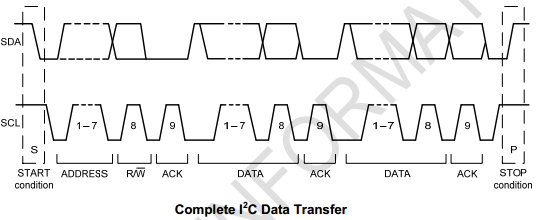
\includegraphics[width=\textwidth*4/5]{../fig/billeder/mpu6050i2c.png}
	\caption{\IIC protokol for MPU-6050}
	\label{fig:mpu6050i2c}
\end{figure}

Som det ses i figur \ref{fig:mpu6050i2c}, starter masteren med at sætte en startsekvens ud på SDA (HIGH-to-LOW), mens SCL er høj. Herefter betragtes bussen som optaget, indtil der bliver sendt en stopsekvens på SDA (LOW-to-HIGH) af masteren, mens SCL ligeledes er høj. Efter startsekvensen bliver der sendt en 7-bits adresse og en R/W bit. Data der bliver transmitteret over \IIC bliver sendt i pakker af 8 bits. Når der først er sendt en startsekvens, er der ingen begrænsning på hvor meget data der må sendes, udover at der efter hver pakke, skal registreres en acknowledge. MPU-6050 indeholder desuden en DMP (Digital Motion Processor), som har til opgave at håndtere noget af dataprocesseringen fra selve MPU-6050. 